\chapter[AWS Deployment]{AWS Deployment\\\small{\textit{-- Charles, Justin, Benedict, Jacky}}}
\label{Chapter::AWS Deployment}
\index{Chapter!AWS Deployment}

\noindent\textbf{Live URL:} \url{https://zjnbvfjpug.us-east-1.awsapprunner.com}

\section*{Overview}
We deployed the \emph{Two Buttons} website as a containerized service on AWS. The pipeline is:
\begin{enumerate}
  \item Authenticate the AWS CLI via \textbf{SSO} (IAM Identity Center).
  \item Build a Docker image locally and push it to \textbf{Amazon ECR}.
  \item Deploy from ECR to a managed container runtime using \textbf{AWS App Runner}.
\end{enumerate}

\paragraph{Why App Runner?}
For a small stateless web app, App Runner removes the need to manage ECS tasks/services, load balancers, or EC2 capacity. It auto-builds or pulls from ECR, provisions HTTPS and scaling, and exposes a public URL with minimal ops overhead (good for a course project).

\paragraph{Project root used for the build}
\path{C:\Users\benma\Documents\docker-examples-benedict\docker-examples\color-buttons-app}

\subsection*{Prerequisites}
\begin{itemize}
  \item Windows 10/11 with \textbf{Docker Desktop} and \textbf{AWS CLI v2}.
  \item \textbf{SSO} set up in the AWS Console (IAM Identity Center) with an AdminAccess permission set (temporary for the lab).
  \item Overleaf configured to compile with \texttt{minted} (shell escape enabled).
\end{itemize}

\section*{Authenticate the AWS CLI (SSO)}
\begin{minted}[fontsize=\small]{powershell}
aws configure sso
aws sso login --profile default
aws sts get-caller-identity --profile default
# Confirm the returned Account ID is yours and an SSO role is assumed.
\end{minted}

\section*{Build, Tag, and Push the Image to Amazon ECR}
\vspace{-0.5\baselineskip}
\begin{minted}[fontsize=\small]{powershell}
# Go to the project folder
cd "C:\Users\benma\Documents\docker-examples-benedict\docker-examples\color-buttons-app"

# Environment
$Env:AWS_REGION="us-east-1"
$Env:ECR_REPO="color-buttons-app"
$Env:IMAGE_TAG="v1"
$Env:AWS_ACCOUNT_ID=(aws sts get-caller-identity --query Account --output text --profile default)

# Create the ECR repo if missing
aws ecr describe-repositories --repository-names $Env:ECR_REPO --region $Env:AWS_REGION --profile default *> $null ; if ($LASTEXITCODE -ne 0) {
  aws ecr create-repository --repository-name $Env:ECR_REPO `
    --image-scanning-configuration scanOnPush=true `
    --region $Env:AWS_REGION --profile default
}

# Log in Docker to ECR
aws ecr get-login-password --region $Env:AWS_REGION --profile default |
  docker login --username AWS --password-stdin "$($Env:AWS_ACCOUNT_ID).dkr.ecr.$($Env:AWS_REGION).amazonaws.com"

# Build, tag, and push (force linux/amd64 for App Runner build fleet compatibility)
docker build --platform linux/amd64 -t "$($Env:ECR_REPO):$($Env:IMAGE_TAG)" .
docker tag  "$($Env:ECR_REPO):$($Env:IMAGE_TAG)" `
            "$($Env:AWS_ACCOUNT_ID).dkr.ecr.$($Env:AWS_REGION).amazonaws.com/$($Env:ECR_REPO):$($Env:IMAGE_TAG)"
docker push "$($Env:AWS_ACCOUNT_ID).dkr.ecr.$($Env:AWS_REGION).amazonaws.com/$($Env:ECR_REPO):$($Env:IMAGE_TAG)"
\end{minted}

\section*{Deploy with AWS App Runner (Console)}
\begin{enumerate}
  \item \textbf{Create service} $\rightarrow$ \textbf{Source}: \emph{Container registry} $\rightarrow$ \emph{Amazon ECR}.\\
        Choose repository \texttt{color-buttons-app} and tag \texttt{v1}.
  \item \textbf{Service name}: \texttt{color-buttons-app} \quad \textbf{Port}: \texttt{3000}.
  \item \textbf{ECR access role}: \emph{Create new service role} (let App Runner pull from ECR).
  \item \textbf{Health check}: \texttt{HTTP} on path \texttt{/} (timeout 5s, interval 10s).
  \item Click \textbf{Create \& Deploy}; wait for \emph{Status: Running} and note the \emph{Default domain}.
\end{enumerate}

\section*{Verification}
\begin{minted}[fontsize=\small]{powershell}
# Expect HTTP/2 200 (or similar)
curl -I https://zjnbvfjpug.us-east-1.awsapprunner.com
\end{minted}
Manually verify the page renders and both buttons switch background color (blue/red).

\section*{Operating the Service (Logs, Scaling, Rollback)}
\begin{itemize}
  \item \textbf{Logs:} In App Runner $\rightarrow$ \emph{Logs} tab to view system/app logs.
  \item \textbf{Scaling:} Default concurrency is 100 requests/instance, min 1, max 25 instances.
  \item \textbf{Re-deploy:} Push the same tag and choose \emph{Actions $\rightarrow$ Deploy} for manual trigger services.
  \item \textbf{Rollback:} Keep prior image tags; re-point the service to the last known-good tag and redeploy.
\end{itemize}

\section*{Cost Guardrails \& Cleanup}
App Runner and ECR are pay-as-you-go. To avoid charges after grading:
\begin{enumerate}
  \item In \textbf{App Runner}: \emph{Actions $\rightarrow$ Pause} or \emph{Delete} the service.
  \item In \textbf{ECR}: delete the image(s) and (optionally) the repository.
\end{enumerate}
(We also set an AWS Budget alarm earlier to notify on any unexpected spend.)

\section*{Figure}
\begin{figure}[htbp]
  \centering
  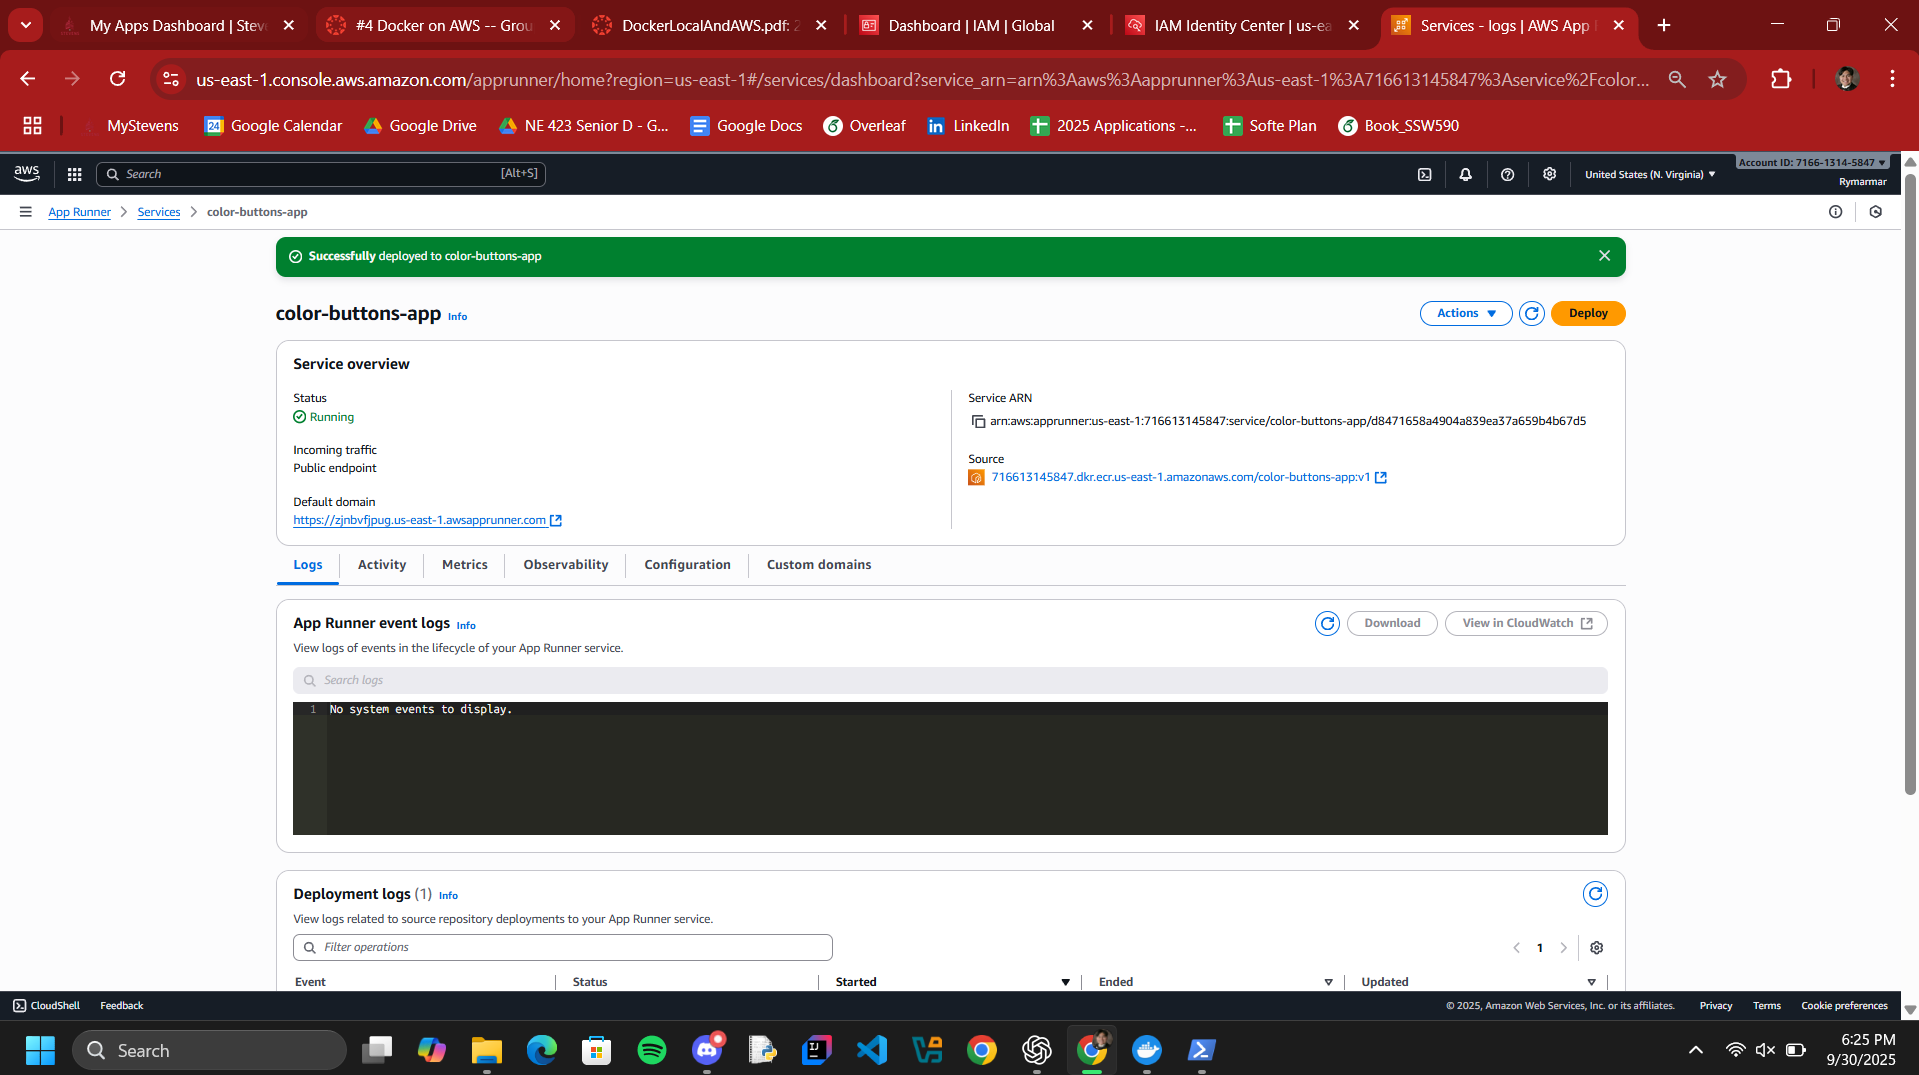
\includegraphics[width=.95\linewidth]{png/docker/app-runner-running.png}
  \caption{App Runner service in \emph{Running} state with the default domain.}
\end{figure}

\section*{Class-based JavaScript Refactor}

We replaced the old function-based handlers with an class that encapsulates all behavior (buttons, events, and background updates). Only the public assets changed (\texttt{public/index.html}, \texttt{public/app.js}); the server continues to serve \texttt{public/} and listen on \texttt{0.0.0.0:3000}.

\subsection*{Updated \texttt{public/index.html}}
\begin{minted}[fontsize=\small]{html}
<!doctype html>
<html lang="en">
<head>
  <meta charset="utf-8" />
  <title>Two Buttons</title>
</head>
<body>
  <h1>Two Buttons</h1>
  <button id="blueBtn">Blue</button>
  <button id="redBtn">Red</button>

  <script src="app.js"></script>
</body>
</html>
\end{minted}

\subsection*{New \texttt{public/app.js} (class-based)}
\begin{minted}[fontsize=\small]{javascript}
class ColorButtonsApp {
  constructor() {
    this.$blue = document.getElementById("blueBtn");
    this.$red  = document.getElementById("redBtn");
    this.bindEvents();
  }
  bindEvents() {
    this.$blue.addEventListener("click", () => this.setBg("steelblue"));
    this.$red .addEventListener("click", () => this.setBg("crimson"));
  }
  setBg(color) { document.body.style.backgroundColor = color; }
}
window.addEventListener("DOMContentLoaded", () => new ColorButtonsApp());
\end{minted}

\begin{figure}[htbp]
  \centering
  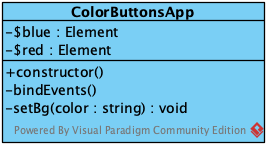
\includegraphics[width=.95\linewidth]{png/docker/DockerOnAWSGroup.png}
  \caption{Class Diagram for App.js}
\end{figure}

\subsection*{Server.js}
\begin{minted}[fontsize=\small]{javascript}
import express from "express";
import path from "path";
import { fileURLToPath } from "url";

const __filename = fileURLToPath(import.meta.url);
const __dirname = path.dirname(__filename);

const app = express();
const PORT = process.env.PORT || 3000;

// Serve static files from public/
app.use(express.static(path.join(__dirname, "public")));

app.listen(PORT, "0.0.0.0", () => {
  console.log(`Server running at http://0.0.0.0:${PORT}!`);
});
\end{minted}

\subsection*{\texttt{package.json}}
\begin{minted}[fontsize=\small]{json}
{
  "name": "color-buttons-app",
  "version": "1.0.0",
  "type": "module",
  "main": "server.js",
  "scripts": {
    "start": "node server.js"
  },
  "dependencies": {
    "express": "^4.18.2"
  }
}
\end{minted}

\paragraph{Result.}
Clicking \textbf{Blue} or \textbf{Red} now triggers methods on a single \texttt{ColorButtonsApp} instance, keeping the global scope clean and making the behavior easy to unit test or extend.
